% answers.tex —— 1978 年·全国卷 · 参考答案与详细解析片段
% 由 tools/generate_projects.py 依来源总账自 1978/1978_数学真题_全国_试题.md + 1978/1978_数学真题_全国_解析正文.md + 1978/1978_数学真题_全国_答案要点.md 生成，勿手改（改源 MD 后重跑）


\begin{gknotice}
\textbf{解析归属}：本卷为文理合卷，原卷仅题面、无答案页。下列解析由本库逐题独立推导并复算，不声称代表官方发布的标准答案。

\textbf{来源说明}：原卷文件名标注“5、6 选做一题，文科不做第 7 题”，即第 5、6 两题卷内二选一，第 7 题文科不作。本解析对 7 题全部给出推导。

\textbf{编注}：第 2 题原卷“内形”当为“形状”之排印误，已如实转录于题面，解析按“形状”理解。
\end{gknotice}

\begin{answer}
\gksolhead{1}{}

\textbf{题目}：

（1） 分解因式：$x^2-4xy+4y^2-4z^2$。

（2） 已知正方形的边长为 $a$，求侧面积等于这个正方形的面积，高等于这个正方形边长的直圆柱体的体积。

（3） 求函数 $y=\sqrt{\lg(2+x)}$ 的定义域。

（4） 不查表求 $\cos 80^\circ\cos 35^\circ+\cos 10^\circ\cos 55^\circ$ 的值。

\Needspace{5\baselineskip}
（5） 化简
\nopagebreak[4]
\[
\left(\frac14\right)^{-\frac12}\cdot\frac{\left(\sqrt{4ab^{-1}}\right)^3}{(0.1)^{-2}\left(a^3b^{-4}\right)^{\frac12}}.
\]

\Needspace{4\baselineskip}
\textbf{解析}

\gksubpart{（1）}

\Needspace{5\baselineskip}
前两项与第三项恰构成完全平方：
\nopagebreak[4]
\[
x^2-4xy+4y^2-4z^2=(x-2y)^2-(2z)^2=(x-2y+2z)(x-2y-2z).
\]
展开复核：$(x-2y)^2-(2z)^2=x^2-4xy+4y^2-4z^2$，与原式一致。

\gksubpart{（2）}

\Needspace{5\baselineskip}
设直圆柱底面半径为 $r$，高为 $h$。由题意 $h=a$，且侧面积等于正方形面积 $a^2$：
\nopagebreak[4]
\[
2\pi rh=a^2\ \Rightarrow\ 2\pi ra=a^2\ \Rightarrow\ r=\frac{a}{2\pi}.
\]
\Needspace{5\baselineskip}
体积为
\nopagebreak[4]
\[
V=\pi r^2h=\pi\left(\frac{a}{2\pi}\right)^2a=\frac{a^3}{4\pi}.
\]
量纲复核：分子 $a^3$、分母 $4\pi$ 无量纲，结果为长度立方，合理。

\gksubpart{（3）}

\Needspace{5\baselineskip}
要使 $y=\sqrt{\lg(2+x)}$ 有意义，须被开方式非负：
\nopagebreak[4]
\[
\lg(2+x)\ge0\iff 2+x\ge1\iff x\ge-1.
\]
定义域为 $[-1,+\infty)$。取边界 $x=-1$ 时 $\lg1=0$、$\sqrt0=0$，确在定义域内；$x<-1$ 时 $\lg(2+x)<0$，根式无意义。

\gksubpart{（4）}

\Needspace{5\baselineskip}
利用余角关系 $\cos10^\circ=\sin80^\circ$、$\cos55^\circ=\sin35^\circ$，原式为
\nopagebreak[4]
\[
\cos80^\circ\cos35^\circ+\sin80^\circ\sin35^\circ=\cos(80^\circ-35^\circ)=\cos45^\circ=\frac{\sqrt2}{2}.
\]
数值复核：$\cos80^\circ\cos35^\circ\approx0.17365\times0.81915\approx0.14224$，$\cos10^\circ\cos55^\circ\approx0.98481\times0.57358\approx0.56486$，两者之和 $\approx0.70710=\dfrac{\sqrt2}{2}$。

\gksubpart{（5）}

\Needspace{5\baselineskip}
逐项化简：
\nopagebreak[4]
\[
\left(\frac14\right)^{-\frac12}=4^{\frac12}=2,\qquad (0.1)^{-2}=10^2=100,
\]
\nopagebreak[4]
\[
\left(\sqrt{4ab^{-1}}\right)^3=\left(4ab^{-1}\right)^{\frac32}=8a^{\frac32}b^{-\frac32},\qquad
\left(a^3b^{-4}\right)^{\frac12}=a^{\frac32}b^{-2}.
\]
\Needspace{5\baselineskip}
于是原式
\nopagebreak[4]
\[
=2\cdot\frac{8a^{\frac32}b^{-\frac32}}{100\,a^{\frac32}b^{-2}}
=2\cdot\frac{8}{100}\,b^{\frac12}=\frac{4}{25}\sqrt b.
\]
取 $a=b=1$ 复算：原式 $=2\cdot\dfrac{2^3}{100\cdot1}=\dfrac{16}{100}=\dfrac{4}{25}$，与化简结果 $\dfrac{4}{25}\sqrt1=\dfrac{4}{25}$ 一致。

\gkanswer{答案（1）：$(x-2y+2z)(x-2y-2z)$}

\gkanswer{答案（2）：$\dfrac{a^3}{4\pi}$}

\gkanswer{答案（3）：$x\ge-1$（即 $[-1,+\infty)$）}

\gkanswer{答案（4）：$\dfrac{\sqrt2}{2}$}

\gkanswer{答案（5）：$\dfrac{4}{25}\sqrt b$}

\end{answer}
\begin{answer}
\gksolhead{2}{}

\textbf{题目}：

已知方程 $kx^2+y^2=4$，其中 $k$ 为实数。对于不同范围的 $k$ 值，分别指出方程所代表图形的内形，并画出显示其数量特征的草图。

\Needspace{4\baselineskip}
\textbf{解析}

方程 $kx^2+y^2=4$ 随参数 $k$ 取值不同而表示不同类型的曲线，需按 $k$ 的符号与 $1$ 的大小分档讨论。

\Needspace{5\baselineskip}
当 $k>0$ 时化为标准椭圆
\nopagebreak[4]
\[
\frac{x^2}{4/k}+\frac{y^2}{4}=1,
\]
其顶点在坐标轴上。比较两半轴：$0<k<1$ 时 $\dfrac4k>4$，长轴在 $x$ 轴；$k=1$ 时方程即 $x^2+y^2=4$，是以原点为心、半径 $2$ 的圆；$k>1$ 时 $\dfrac4k<4$，长轴在 $y$ 轴。草图应标出顶点坐标（$\pm2/\sqrt k$ 与 $\pm2$）。

当 $k=0$ 时方程退化为 $y^2=4$，即 $y=2$ 与 $y=-2$ 两条平行直线，草图为两条相距 $4$ 的水平线。

\Needspace{5\baselineskip}
当 $k<0$ 时，记 $k=-c$（$c>0$），方程化为
\nopagebreak[4]
\[
\frac{y^2}{4}-\frac{x^2}{4/c}=1,
\]
是以 $y$ 轴为实轴的双曲线，顶点为 $(0,\pm2)$。特例 $k=-1$ 时为等轴双曲线 $y^2-x^2=4$。

\gkanswer{答案：$k>0$ 时为椭圆（$0<k<1$ 时长轴在 $x$ 轴，$k=1$ 时为圆 $x^2+y^2=4$，$k>1$ 时长轴在 $y$ 轴）；$k=0$ 时为两条平行直线 $y=\pm2$；$k<0$ 时为双曲线（焦点在 $y$ 轴）}

\end{answer}
\begin{answer}
\gksolhead{3}{}

\textbf{题目}：

如图，$AB$ 是半圆的直径，$C$ 是半圆上一点，直线 $MN$ 切半圆于 $C$ 点，$AM\perp MN$ 于 $M$ 点，$BN\perp MN$ 于 $N$ 点，$CD\perp AB$ 于 $D$ 点。求证：

（1） $CD=CM=CN$；

（2） $CD^2=AM\cdot BN$。
\nopagebreak[4]
\begin{center}% 1978 年全国卷第 3 题：半圆（直径 AB），C 在弧上，MN 切半圆于 C，AM⊥MN 于 M、BN⊥MN 于 N、CD⊥AB 于 D（按源卷布局）
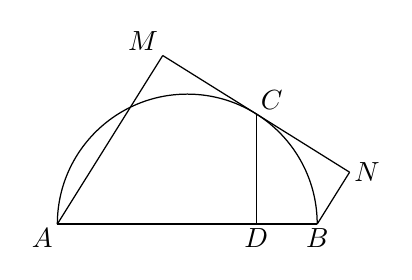
\begin{tikzpicture}[scale=1.65, line width=0.45pt,
  every node/.style={inner sep=1.5pt}]
  \coordinate (A) at (-1,0);
  \coordinate (B) at (1,0);
  \coordinate (C) at (0.53,0.848);
  \coordinate (D) at (0.53,0);
  \coordinate (M) at (-0.189,1.297);
  \coordinate (N) at (1.249,0.399);
  \draw (A) arc (180:0:1);
  \draw (A) -- (B);
  \draw (M) -- (N);
  \draw (A) -- (M);
  \draw (B) -- (N);
  \draw (C) -- (D);
  \node[anchor=south east] at (M) {$M$};
  \node[anchor=south west] at (C) {$C$};
  \node[anchor=west] at (N) {$N$};
  \node[anchor=north east] at (A) {$A$};
  \node[anchor=north] at (D) {$D$};
  \node[anchor=north] at (B) {$B$};
\end{tikzpicture}
\end{center}
\nopagebreak[4]
\Needspace{4\baselineskip}
\textbf{解析}
\nopagebreak[4]
\begin{center}% 1978 年全国卷第 3 题：半圆（直径 AB），C 在弧上，MN 切半圆于 C，AM⊥MN 于 M、BN⊥MN 于 N、CD⊥AB 于 D（按源卷布局）
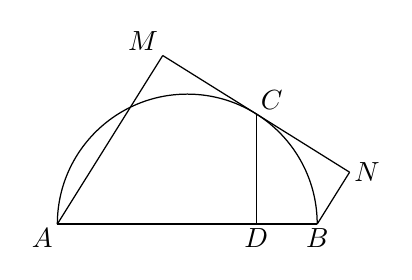
\begin{tikzpicture}[scale=1.65, line width=0.45pt,
  every node/.style={inner sep=1.5pt}]
  \coordinate (A) at (-1,0);
  \coordinate (B) at (1,0);
  \coordinate (C) at (0.53,0.848);
  \coordinate (D) at (0.53,0);
  \coordinate (M) at (-0.189,1.297);
  \coordinate (N) at (1.249,0.399);
  \draw (A) arc (180:0:1);
  \draw (A) -- (B);
  \draw (M) -- (N);
  \draw (A) -- (M);
  \draw (B) -- (N);
  \draw (C) -- (D);
  \node[anchor=south east] at (M) {$M$};
  \node[anchor=south west] at (C) {$C$};
  \node[anchor=west] at (N) {$N$};
  \node[anchor=north east] at (A) {$A$};
  \node[anchor=north] at (D) {$D$};
  \node[anchor=north] at (B) {$B$};
\end{tikzpicture}
\end{center}
\nopagebreak[4]
\Needspace{5\baselineskip}
设半圆圆心为 $O$，半径为 $R$，连 $OC$。因 $MN$ 与半圆相切于 $C$，故 $OC\perp MN$；又 $AM\perp MN$、$BN\perp MN$，所以
\nopagebreak[4]
\[
AM\parallel OC\parallel BN.
\]

\gksubpart{（1）}

\Needspace{5\baselineskip}
先证 $CM=CD$。由 $\angle AMC=90^\circ$、$\angle ADC=90^\circ$，$A$、$M$、$C$、$D$ 四点共圆，直径 $AC$。该圆中弦 $CM$、$CD$ 分别被顶点 $A$ 处的圆周角 $\angle CAM$、$\angle CAD$ 所对，故只需比较这两角：
\nopagebreak[4]
\[
\angle CAM=\angle ACO\quad(\text{因 }AM\parallel OC),
\]
又 $OA=OC$，三角形 $AOC$ 等腰，$\angle ACO=\angle CAO=\angle CAD$（$D$ 在 $AB$ 上），于是 $\angle CAM=\angle CAD$，得 $CM=CD$。

\Needspace{5\baselineskip}
再证 $CN=CD$。由 $\angle BNC=90^\circ$、$\angle BDC=90^\circ$，$B$、$N$、$C$、$D$ 四点共圆，直径 $BC$。弦 $CN$、$CD$ 分别被顶点 $B$ 处的圆周角 $\angle CBN$、$\angle CBD$ 所对，而
\nopagebreak[4]
\[
\angle CBN=\angle BCO\quad(\text{因 }BN\parallel OC),
\]
又 $OB=OC$，$\angle BCO=\angle CBO=\angle CBD$，于是 $\angle CBN=\angle CBD$，得 $CN=CD$。

综上 $CD=CM=CN$。

\gksubpart{（2）}

\Needspace{5\baselineskip}
在圆 $AMCD$ 中，$\angle AMD$ 与 $\angle ACD$ 同对弦 $AD$，故 $\angle AMD=\angle ACD=90^\circ-\angle CAD$；又 $\angle MDA$ 与 $\angle MCA$ 同对弦 $MA$，故 $\angle MDA=\angle MCA$，而由切线弦角定理（$MC$ 切于 $C$）
\nopagebreak[4]
\[
\angle MCA=\angle CBA=90^\circ-\angle CAD.
\]
\Needspace{5\baselineskip}
所以 $\angle AMD=\angle MDA$，三角形 $AMD$ 中两底角相等，得
\nopagebreak[4]
\[
AM=AD.
\]
\Needspace{5\baselineskip}
同法在圆 $BNCD$ 中：$\angle BND=\angle BCD=90^\circ-\angle CBA$，$\angle BDN=\angle BCN=\angle CAB$，而 $90^\circ-\angle CBA=\angle CAB$，故 $\angle BND=\angle BDN$，得
\nopagebreak[4]
\[
BN=BD.
\]
\Needspace{5\baselineskip}
因此
\nopagebreak[4]
\[
AM\cdot BN=AD\cdot DB.
\]
\Needspace{5\baselineskip}
另一方面，$AB$ 是直径故 $\angle ACB=90^\circ$，$CD$ 是直角三角形 $ACB$ 斜边 $AB$ 上的高，由射影定理
\nopagebreak[4]
\[
CD^2=AD\cdot DB.
\]
两式联立即得 $CD^2=AM\cdot BN$。

\gkanswer{答案（1）：见解析版}

\gkanswer{答案（2）：见解析版}

\end{answer}
\begin{answer}
\gksolhead{4}{}

\textbf{题目}：

已知 $\log_{18}9=a$，$18^b=5$，求 $\log_{36}45$。

\Needspace{4\baselineskip}
\textbf{解析}

由 $18^b=5$ 取以 $18$ 为底的对数，得 $b=\log_{18}5$，又已知 $a=\log_{18}9$。

\Needspace{5\baselineskip}
所求对数的分子：
\nopagebreak[4]
\[
\log_{18}45=\log_{18}(9\times5)=\log_{18}9+\log_{18}5=a+b.
\]
\Needspace{5\baselineskip}
分母：
\nopagebreak[4]
\[
\log_{18}36=\log_{18}(18\times2)=1+\log_{18}2=1+\log_{18}\frac{18}{9}=1+(1-a)=2-a.
\]
\Needspace{5\baselineskip}
于是
\nopagebreak[4]
\[
\log_{36}45=\frac{\log_{18}45}{\log_{18}36}=\frac{a+b}{2-a}.
\]
数值复核：$a\approx0.76019$，$b\approx0.55681$，$\dfrac{a+b}{2-a}\approx\dfrac{1.31700}{1.23981}\approx1.06227$，而直接计算 $\dfrac{\ln45}{\ln36}\approx\dfrac{3.80666}{3.58352}\approx1.06225$，一致。

\gkanswer{答案：$\dfrac{a+b}{2-a}$}

\end{answer}
\begin{answer}
\gksolhead{5}{}

\textbf{题目}：

已知 $\triangle ABC$ 的三个内角的大小成等差数列，$\tan A\tan C=2+\sqrt3$，求角 $A$、$B$、$C$ 的大小。又已知顶点 $C$ 的对边 $c$ 上的高等于 $4\sqrt3$，求三角形各边 $a$、$b$、$c$ 的长。（提示：必要时可验证 $(1+\sqrt3)^2=4+2\sqrt3$）

\Needspace{4\baselineskip}
\textbf{解析}

\Needspace{5\baselineskip}
三内角成等差数列，可设 $A+C=2B$；又 $A+B+C=180^\circ$，故 $3B=180^\circ$，得
\nopagebreak[4]
\[
B=60^\circ,\qquad C=120^\circ-A.
\]
\Needspace{5\baselineskip}
设 $x=\tan A$，由两角和正切公式
\nopagebreak[4]
\[
\tan C=\tan(120^\circ-A)=\frac{-\sqrt3-x}{1-\sqrt3x}.
\]
\Needspace{5\baselineskip}
代入 $\tan A\tan C=2+\sqrt3$：
\nopagebreak[4]
\[
x\cdot\frac{-\sqrt3-x}{1-\sqrt3x}=2+\sqrt3
\ \Longrightarrow\ -\sqrt3x-x^2=(2+\sqrt3)(1-\sqrt3x).
\]
\Needspace{5\baselineskip}
右边展开 $(2+\sqrt3)(1-\sqrt3x)=(2+\sqrt3)-(2\sqrt3+3)x$，移项整理得
\nopagebreak[4]
\[
x^2-(3+\sqrt3)x+(2+\sqrt3)=0.
\]
\Needspace{5\baselineskip}
判别式
\nopagebreak[4]
\[
\Delta=(3+\sqrt3)^2-4(2+\sqrt3)=12+6\sqrt3-8-4\sqrt3=4+2\sqrt3=(1+\sqrt3)^2
\]
\Needspace{5\baselineskip}
（与题给提示吻合），故
\nopagebreak[4]
\[
x=\frac{(3+\sqrt3)\pm(1+\sqrt3)}{2},
\]
\Needspace{5\baselineskip}
即 $x=2+\sqrt3$ 或 $x=1$，对应 $A=75^\circ$ 或 $A=45^\circ$。于是
\nopagebreak[4]
\[
B=60^\circ,\qquad (A,C)=(45^\circ,75^\circ)\ \text{或}\ (75^\circ,45^\circ).
\]
复核：$1\cdot\tan75^\circ=2+\sqrt3$，满足题设。

\Needspace{5\baselineskip}
再求边。设 $c$ 边（即 $AB$）上的高为 $h_c=4\sqrt3$。由 $h_c=a\sin B$，
\nopagebreak[4]
\[
a=\frac{4\sqrt3}{\sin60^\circ}=\frac{4\sqrt3}{\sqrt3/2}=8.
\]
由 $h_c=b\sin A$：
\begin{itemize}
\item 若 $A=45^\circ$，$\sin A=\dfrac{\sqrt2}{2}$，$b=\dfrac{4\sqrt3}{\sqrt2/2}=4\sqrt6$；
\item 若 $A=75^\circ$，$b=\dfrac{4\sqrt3}{\sin75^\circ}=\dfrac{4\sqrt3\cdot4}{\sqrt6+\sqrt2}=\dfrac{16\sqrt3(\sqrt6-\sqrt2)}{4}=4\sqrt3(\sqrt6-\sqrt2)=12\sqrt2-4\sqrt6$。
\end{itemize}

由正弦定理 $c=\dfrac{a\sin C}{\sin A}$：
\begin{itemize}
\item 若 $(A,C)=(45^\circ,75^\circ)$，$c=8\cdot\dfrac{\sin75^\circ}{\sin45^\circ}=8\cdot\dfrac{(\sqrt6+\sqrt2)/4}{\sqrt2/2}=4(\sqrt3+1)=4+4\sqrt3$；
\item 若 $(A,C)=(75^\circ,45^\circ)$，$c=8\cdot\dfrac{\sin45^\circ}{\sin75^\circ}=\dfrac{16\sqrt2}{\sqrt6+\sqrt2}=\dfrac{16\sqrt2(\sqrt6-\sqrt2)}{4}=4(2\sqrt3-2)=8\sqrt3-8$。
\end{itemize}

复算：两种情形均有 $a=8$。正弦定理比值 $\dfrac{a}{\sin A}$：第一种 $8\sqrt2\approx11.314$，且 $\dfrac{b}{\sin B}=\dfrac{4\sqrt6}{\sqrt3/2}=8\sqrt2$、$\dfrac{c}{\sin C}\approx11.314$ 三值相等；第二种 $\dfrac{8}{\sin75^\circ}\approx8.282$，$\dfrac{12\sqrt2-4\sqrt6}{\sqrt3/2}\approx8.282$、$\dfrac{8\sqrt3-8}{\sqrt2/2}\approx8.282$ 亦相等。高线复核：第一种 $b\sin A=4\sqrt6\cdot\dfrac{\sqrt2}{2}=4\sqrt3$；第二种 $(12\sqrt2-4\sqrt6)\sin75^\circ\approx6.928=4\sqrt3$，均符合题设。

\gkanswer{答案：$B=60^\circ$，$(A,C)=(45^\circ,75^\circ)$ 或 $(75^\circ,45^\circ)$。当 $(A,C)=(45^\circ,75^\circ)$ 时 $a=8$、$b=4\sqrt6$、$c=4+4\sqrt3$；当 $(A,C)=(75^\circ,45^\circ)$ 时 $a=8$、$b=12\sqrt2-4\sqrt6$、$c=8\sqrt3-8$}

\end{answer}
\begin{answer}
\gksolhead{6}{}

\textbf{题目}：

\Needspace{5\baselineskip}
已知 $\alpha$、$\beta$ 为锐角，$3\sin^2\alpha+2\sin^2\beta=1$，$3\sin 2\alpha-2\sin 2\beta=0$。求证：
\nopagebreak[4]
\[
\alpha+2\beta=\frac{\pi}{2}.
\]

\Needspace{4\baselineskip}
\textbf{解析}

\Needspace{5\baselineskip}
由第一个条件，注意 $1-2\sin^2\beta=\cos2\beta$：
\nopagebreak[4]
\[
2\sin^2\beta=1-3\sin^2\alpha\ \Longrightarrow\ \cos2\beta=1-2\sin^2\beta=3\sin^2\alpha. \tag{i}
\]
\Needspace{5\baselineskip}
由第二个条件 $3\sin2\alpha=2\sin2\beta$，即
\nopagebreak[4]
\[
\sin2\beta=\frac32\sin2\alpha=3\sin\alpha\cos\alpha. \tag{ii}
\]
\Needspace{5\baselineskip}
把 (i)(ii) 两式平方相加：
\nopagebreak[4]
\[
\cos^22\beta+\sin^22\beta=9\sin^4\alpha+9\sin^2\alpha\cos^2\alpha=9\sin^2\alpha(\sin^2\alpha+\cos^2\alpha)=9\sin^2\alpha.
\]
左端恒为 $1$，故 $9\sin^2\alpha=1$，$\sin\alpha=\dfrac13$（$\alpha$ 为锐角，取正）。

\Needspace{5\baselineskip}
代回得
\nopagebreak[4]
\[
\cos2\beta=3\cdot\frac19=\frac13=\sin\alpha,\qquad
\sin2\beta=3\cdot\frac13\cdot\frac{2\sqrt2}{3}=\frac{2\sqrt2}{3}=\cos\alpha.
\]
\Needspace{5\baselineskip}
因 $\beta$ 为锐角，$0<2\beta<\pi$，而 $\cos2\beta=\dfrac13>0$，故 $0<2\beta<\dfrac\pi2$；同理 $0<\dfrac\pi2-\alpha<\dfrac\pi2$。两角都在余弦函数单调递减的区间内且余弦值相等，所以
\nopagebreak[4]
\[
2\beta=\frac\pi2-\alpha,
\]
即 $\alpha+2\beta=\dfrac\pi2$。

数值复核：$\sin\alpha=\dfrac13\Rightarrow\alpha\approx19.471^\circ$，$\cos2\beta=\dfrac13\Rightarrow2\beta\approx70.529^\circ$，两者之和恰为 $90^\circ$；代入原式 $3\sin^2\alpha\approx0.3333$、$2\sin^2\beta\approx0.6667$ 和为 $1$，$3\sin2\alpha\approx1.8856$、$2\sin2\beta\approx1.8856$ 相等。

\gkanswer{答案：见解析版}

\end{answer}
\begin{answer}
\gksolhead{7}{}

\textbf{题目}：

已知函数 $y=x^2+(2m+1)x+m^2-1$（$m$ 为实数）。

（1） $m$ 是什么数值时，$y$ 的极值是 $0$？

（2） 求证：不论 $m$ 是什么数值，函数图象（即抛物线）的顶点都在同一条直线 $L_1$ 上，画出 $m=-1$、$0$、$1$ 时抛物线的草图，来检验这个结论；

（3） 平行于 $L_1$ 的直线中，哪些与抛物线相交，哪些不相交？求证：任一条平行于 $L_1$ 而与抛物线相交的直线，被各抛物线截出的线段都相等。

\Needspace{4\baselineskip}
\textbf{解析}

\gksubpart{（1）}

\Needspace{5\baselineskip}
配方求顶点。函数的顶点横坐标为
\nopagebreak[4]
\[
x_v=-\frac{2m+1}{2},
\]
\Needspace{5\baselineskip}
代入得最小值
\nopagebreak[4]
\[
y_v=m^2-1-\frac{(2m+1)^2}{4}=\frac{4m^2-4-(4m^2+4m+1)}{4}=-\frac{4m+5}{4}.
\]
\Needspace{5\baselineskip}
令 $y_v=0$，得
\nopagebreak[4]
\[
4m+5=0\ \Longrightarrow\ m=-\frac54.
\]
复核 $m=-\dfrac54$：此时 $2m+1=-\dfrac32$，$x_v=\dfrac34$，$y_v=\dfrac9{16}-\dfrac32\cdot\dfrac34+\dfrac{25}{16}-1=0$，符合。

\gksubpart{（2）}

\Needspace{5\baselineskip}
顶点坐标为
\nopagebreak[4]
\[
\left(-\frac{2m+1}{2},\ -\frac{4m+5}{4}\right)=\left(-m-\frac12,\ -m-\frac54\right).
\]
\Needspace{5\baselineskip}
两坐标之差
\nopagebreak[4]
\[
y_v-x_v=\left(-m-\frac54\right)-\left(-m-\frac12\right)=-\frac34
\]
\Needspace{5\baselineskip}
与 $m$ 无关，故顶点恒在直线
\nopagebreak[4]
\[
L_1:\ y=x-\frac34
\]
上。

复核 $m=-1,\ 0,\ 1$：对应的顶点分别为 $\left(\dfrac12,-\dfrac14\right)$、$\left(-\dfrac12,-\dfrac54\right)$、$\left(-\dfrac32,-\dfrac94\right)$，逐一代入 $y=x-\dfrac34$ 均成立；描出这三条抛物线后可见其顶点排列在直线 $L_1$ 上，结论得验。

\gksubpart{（3）}

\Needspace{5\baselineskip}
平行于 $L_1$ 的直线可写成 $y=x+b$。与抛物线联立：
\nopagebreak[4]
\[
x^2+(2m+1)x+m^2-1=x+b
\ \Longrightarrow\ x^2+2mx+(m^2-1-b)=0.
\]
\Needspace{5\baselineskip}
判别式
\nopagebreak[4]
\[
\Delta=(2m)^2-4(m^2-1-b)=4(1+b),
\]
与 $m$ 无关。因此：$b>-1$ 时 $\Delta>0$，直线与每条抛物线交于两点；$b=-1$ 时 $\Delta=0$，相切；$b<-1$ 时 $\Delta<0$，不相交。

\Needspace{5\baselineskip}
相交时两交点横坐标之差
\nopagebreak[4]
\[
|x_2-x_1|=\sqrt{\Delta}=2\sqrt{1+b},
\]
\Needspace{5\baselineskip}
它们落在斜率为 $1$ 的直线上，故截得线段长
\nopagebreak[4]
\[
|x_2-x_1|\sqrt{1^2+1^2}=2\sqrt2\sqrt{1+b},
\]
只与 $b$ 有关，与 $m$ 无关，即任一条平行于 $L_1$ 且与抛物线相交的直线被各抛物线截出的线段都相等。

复核：取 $b=0$（即 $y=x$）、$m=0$，抛物线 $y=x^2+x-1$ 与之交于 $x^2=1$，两点 $(1,1)$、$(-1,-1)$，距离 $2\sqrt2$；取 $m=1$，抛物线 $y=x^2+3x$ 与之交于 $x(x+2)=0$，两点 $(0,0)$、$(-2,-2)$，距离同为 $2\sqrt2$，与公式 $2\sqrt2\sqrt{1+0}$ 一致。

\gkanswer{答案（1）：$m=-\dfrac54$}

\gkanswer{答案（2）：顶点均在直线 $L_1:y=x-\dfrac34$ 上}

\gkanswer{答案（3）：设直线为 $y=x+b$，则 $b\ge-1$ 时与各抛物线都相交（$b=-1$ 时相切），$b<-1$ 时不相交；相交时被每条抛物线截出的线段长均为 $2\sqrt2\sqrt{1+b}$，与 $m$ 无关}

\end{answer}